\newpage % Zaleca się otwieranie rozdziału od nowej strony.
\section{Wstęp teoretyczny}
\label{sc:wstep}
W tym etapie jednym z zaplanowanych celów, było zapoznanie się z teorią stojącą za
kryptografią krzywych eliptycznych. Aby jednak zrozumieć to zagadnienie, musiałem również
zgłębić szersze pole tej dziedziny kryptografii, jaką jest kryptografia oparta o \textbf{problem logarytmu dyskretnego}, zarówno na krzywych eliptycznych jak i innych, odpowiednich grupach.
\newline

\indent
Każde wymienione poniżej zagadnienie, zaimplementowałem również w pakiecie obliczeniowym SageMath. Odpowiadające zaganieniom listingi kodu znajdują się w dalszej części raportu.
\subsection{Problem logarytmu dyskretnego}
Problem logarytmu dyskretnego (\textbf{DLP}) jest podstawą wielu kryptosystemów. Najbardziej znanym z nich jest kryptosystem ElGamala. Problem logarytmu dyskretnego
można przedstawić zarówno na grupie multiplikatywnej $(\mathbb{G},\cdot)$
oraz grupie addytywnej, przy odpowiednim zdefiniowaniu
operacji dodawania na krzywej eliptycznej $(\mathbb{E},+)$ \cite{stinson21}.

\subsection{DLP w grupie multiplikatywnej}
Jeżeli $\mathbb{G}$ to (skończona) grupa multiplikatywna, $\alpha \in \mathbb{G}$
to element rzędu $n$ oraz $\beta \in \mathbb{<\alpha>}$ (jest w podgrupie generowanej
przez $\alpha$), to uważane za problematyczne jest znalezienie takiej liczby $a$:
\[a \in \mathbb{Z} \textrm{ oraz } 0\le a \le n-1\]
że:
\[\alpha ^ a = \beta\]

Liczbę $a$ można przedstawić jako:
\[\log_{\alpha}{\beta}\]


\subsection{DLP w grupie addytywnej}
W przypadku krypografii opartej o krzywe eliptyczne, DLP dotyczy
grupy addytywnej $(\mathbb{E},+)$ zdefiniowanej na krzywej eliptycznej.
Niech $\alpha$ jest rzędu n.
W takim przypadku, ponieważ operacją na grupie jest dodawanie modulo n, to działanie
potęgowania przedstawia się jako:
\[\alpha \cdot a = \beta \textrm{ (mod } n)\]
Przy odpowiednim wyborze grupy addytywnej, rozwiązanie problemu logarytmu dyskretnego,
tj. znalezienie $a$,
jest trudne \cite{chrzaszczyk2010}\cite{stinson21}.
\subsection{Krzywe eliptyczne}
Krzywą eliptyczną nieosobliwą nad ciałem $\mathbb{K}$ o charakterystyce różnej od 2 i 3 definiuje się
za jako zbiór rozwiązań $(x,y) \in \mathbb{R} \times \mathbb{R}$ równiania: \cite*{stinson21}
\[y^2 = x^3 + ax + b\]
przy założeniu, że stałe $a, b$ takie, że:
\[4a^3 + 27b^2 \not= 0\]
Jest to tak zwana forma {\it Weierstrassa} krzywej eliptycznej.

\subsubsection{Krzywe eliptyczne na liczbach rzeczywistych}

Krzywe eliptyczne zdefiniowane na liczbach rzeczywistych nie są kluczowe w
systemach kryptograficznych\cite*{chrzaszczyk2010}\cite*{stinson21}, ale takie ustawienia
pozwalają na prostsze przedstawienie niektórych zagadnień
np. dodawnie punktów na krzywej.
\begin{figure}[!h]
    \centering 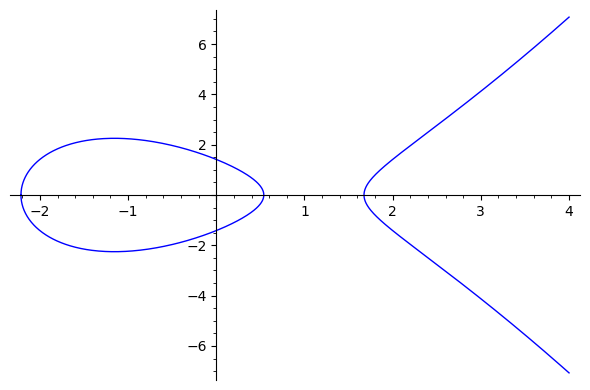
\includegraphics[width=0.8\linewidth]{sage/krzywa_-4_2.png}
    \caption{Krzywa eliptyczna $y^2=x^3-4+2$}
\end{figure}

\subsubsection*{Krzywe eliptyczne na ciele skończonym}
Krzywa eliptyczna na ciele skończonym jest stosowana w kryptografii.
Z powodu charakterystyki ciała, jej wykres
nie przypomina krzywej na liczbach rzeczywistych.
Krzywa taka składa się z punktów, których współrzędne należą do ciała
na którym jest opisana.
Wszystkie operacje na krzywej, takie jak dodawanie, wykonuje się
również z zastosowaniem operacji modulo rzędu ciała.
\begin{figure}[!h]
    \centering 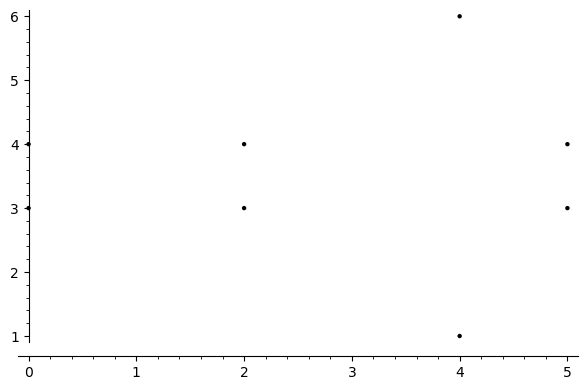
\includegraphics[width=0.8\linewidth]{sage/elliptic_finite_field.png}
    \caption{Krzywa eliptyczna $y^2=x^3-4+2$ nad $GF(7)$}
\end{figure}

\subsubsection{Dodawanie punktów na krzywej eliptycznej}
Przedstwienie krzywej eliptycznej na ciele liczb rzeczywistych,
umożliwia proste zwizualizowanie geometrycznej interpretacji dodawania punktów
leżących na krzywej.
\newline
\indent
Geometryczne dodawanie punktów na krzywej eliptycznej polega na połączeniu
dwóch punktów $P$ i $Q$ prostopadłą linią, która przecina krzywą w trzecim
punkcie, $R'$. Następnie, wynikowy punkt $R$, będący sumą $P+QP+Q$, znajdujemy przez
odbicie punktu $R'$ względem osi $x$. W przypadku dublowania punktu, czyli dodawania
punktu PP do siebie samego, rysujemy styczną do krzywej w punkcie $P$, która przecina
krzywą w nowym punkcie. Odbicie tego punktu względem osi $x$ daje nam wynik $2P$.
\newline
Kod w SageMath użyty do wizualizacji dodawania: listing \ref*{sage_1}
\begin{figure}[!h]
    \centering 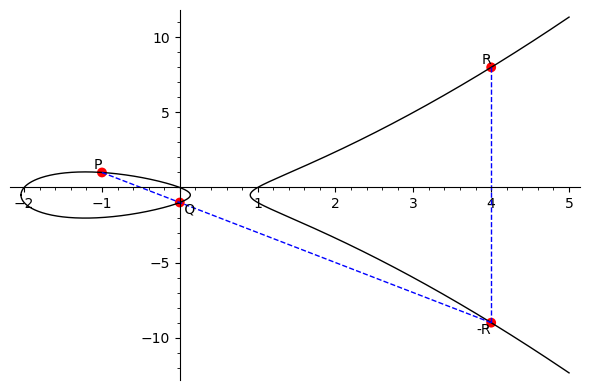
\includegraphics[width=0.8\linewidth]{sage/elliptic_rational_point_addition.png}
    \caption{P + Q na krzywej eliptycznej $y^2+y=x^3-x^2+2x$}
\end{figure}
\newpage

\subsubsection{Dodawanie punktów na krzywej zdefiniowanej na ciele skończonym}
Dodawanie punktów krzywej eliptycznej na ciele skończonym nie ma przejrzyjstej
reprezentacji geometrycznej.
W tym celu stosuje się podejście analityczne.
Wtedy, dodawanie wygląda w następujący sposób:
\begin{enumerate}
    \item Przypadek, gdy \( P \neq Q \):
          \begin{align*}
              \lambda & = \frac{y_2 - y_1}{x_2 - x_1}, \\
              x_3     & = \lambda^2 - x_1 - x_2,       \\
              y_3     & = \lambda(x_1 - x_3) - y_1
          \end{align*}

    \item Przypadek, gdy \( P = Q \):
          \begin{align*}
              \lambda & = \frac{3x_1^2 + a}{2y_1}, \\
              x_3     & = \lambda^2 - 2x_1,        \\
              y_3     & = \lambda(x_1 - x_3) - y_1
          \end{align*}
\end{enumerate}
Dodawanie punktów w SageMath listing \ref{sage_1}

